\documentclass[11pt]{article}

\usepackage[english]{babel}
\usepackage[utf8x]{inputenc}
\usepackage[T1]{fontenc}
\usepackage{helvet}
\usepackage{amsmath}
\usepackage{amssymb}
\usepackage{amsthm}
\usepackage{gensymb}
\usepackage{caption}
\usepackage{enumerate}
\usepackage{enumitem}
\newcommand{\numpy}{{\tt numpy}}    % tt font for numpy
\usepackage[a4paper,top=3cm,bottom=2cm,left=3cm,right=3cm,marginparwidth=1.75cm]{geometry}
\setlength{\arrayrulewidth}{0.5mm}
\setlength{\tabcolsep}{4pt}

\usepackage[colorinlistoftodos]{todonotes}
\usepackage[colorlinks=true, allcolors=blue]{hyperref}
\usepackage{array}
\usepackage{float}
\usepackage{appendix} 
\usepackage{multirow}
\usepackage[symbol]{footmisc}
\usepackage{setspace}
\usepackage{authblk} %%% Support for footnote style author/affiliation.
\usepackage{ctable}
\renewcommand{\arraystretch}{1.3}
\newcommand{\beq}{\begin{equation}}
\newcommand{\eeq}{\end{equation}}

\topmargin -.5in
\textheight 9in
\oddsidemargin -.25in
\evensidemargin -.25in
\textwidth 7in



\title{Classical Mechanics Computational Set}
\author{Antonio Cobarrubia}
\date{}

\begin{document}
\maketitle
\section*{Parametric Curves}
\begin{figure}[H]
    \centering
    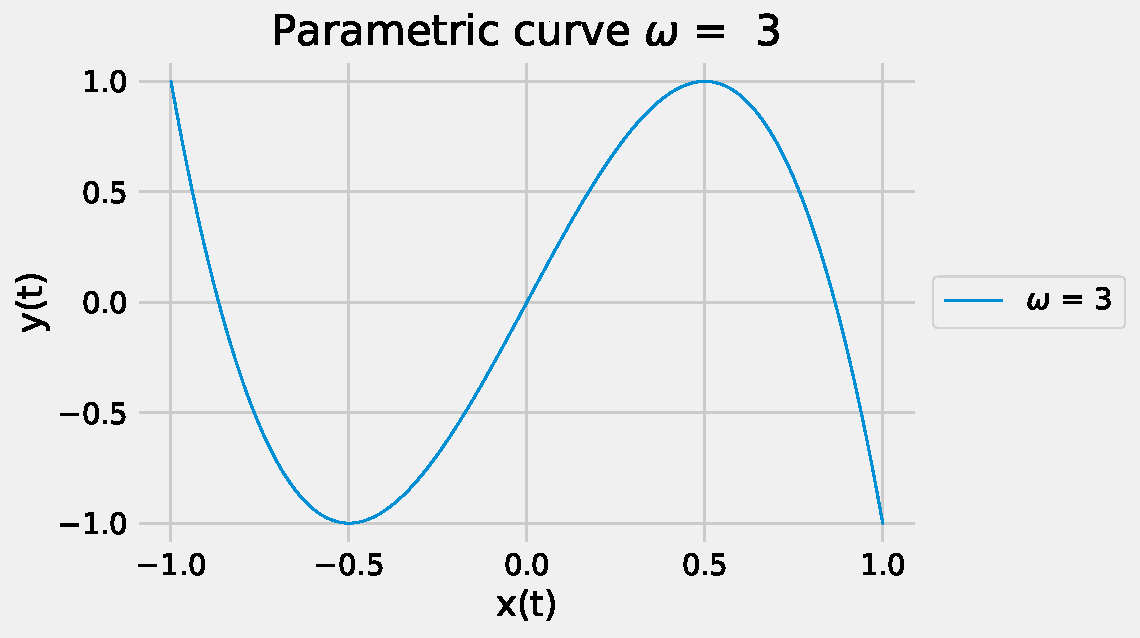
\includegraphics[width = 12 cm]{src/parametricw1.pdf}
    \caption{Lissajous figure with a "frequency" of $\omega = 3$. The frequency is a rational number that shows no interesting dynamical behavior.}
    \label{fig:my_label}
\end{figure}
\begin{figure}[H]
    \centering
    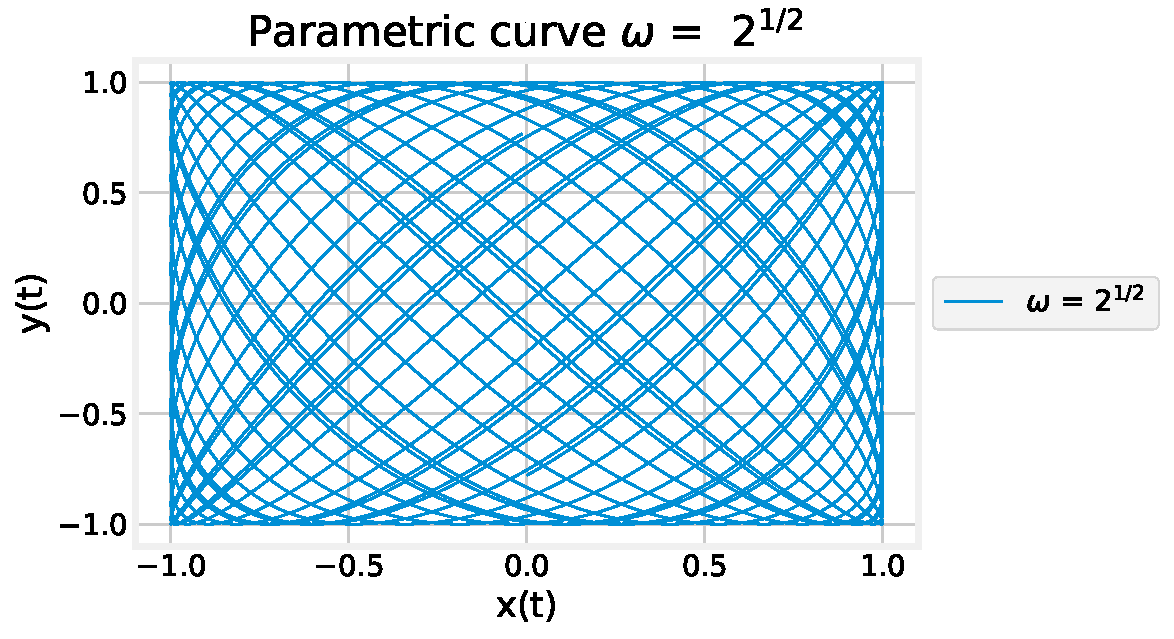
\includegraphics[width = 12 cm]{src/parametricw2.pdf}
    \caption{Lissajous figure with a "frequency" of $\omega = 2^{1/2}$. The frequency is an irrational number that produces interesting dynamical behavior.}
    \label{fig:my_label}
\end{figure}
\begin{figure}[H]
    \centering
    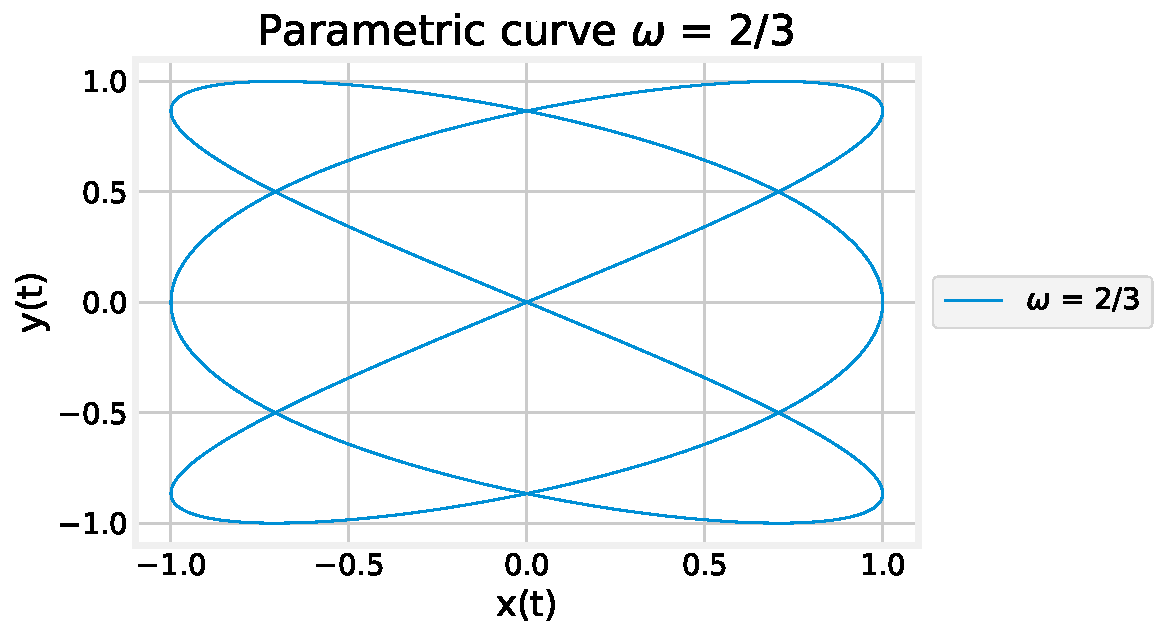
\includegraphics[width = 12 cm]{src/parametricw3.pdf}
    \caption{Lissajous figure with a "frequency" of $\omega = 2/3$ The frequency is a rational number. According to the few Lissajous figures, the trend for these parametric curves seem to explode in behavior with irrational frequencies.  }
    \label{fig:my_label}
\end{figure}
\begin{figure}[H]
    \centering
    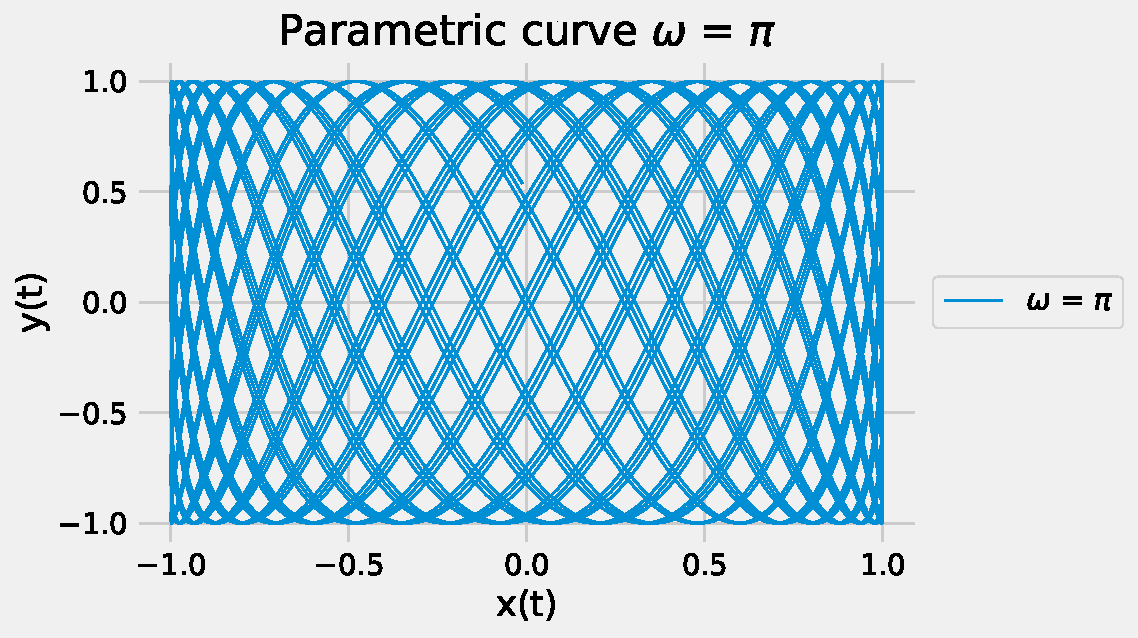
\includegraphics[width = 12 cm]{src/parametricw4.pdf}
    \caption{Lissajous figure with a "frequency" of $\omega = \pi$. The frequency is an irrational number. As suspected, irrational numbers are producing weird dynamical behaviors for these parametric curves.}
    \label{fig:my_label}
\end{figure}\begin{figure}[H]
    \centering
    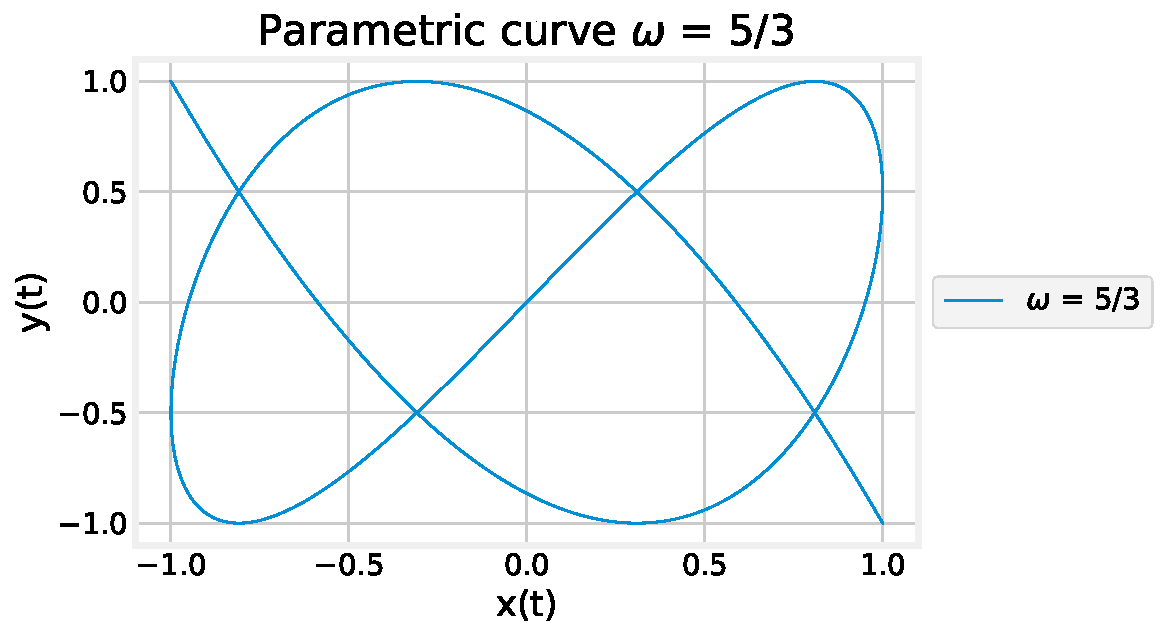
\includegraphics[width = 12 cm]{src/parametricw5.pdf}
    \caption{Lissajous figure with a "frequency" of $\omega = 5/3$ The frequency is a rational number.  Rational numbers seem to converge to some periodic motion after long generations of time. }
    \label{fig:my_label}
\end{figure}
\begin{figure}[H]
    \centering
    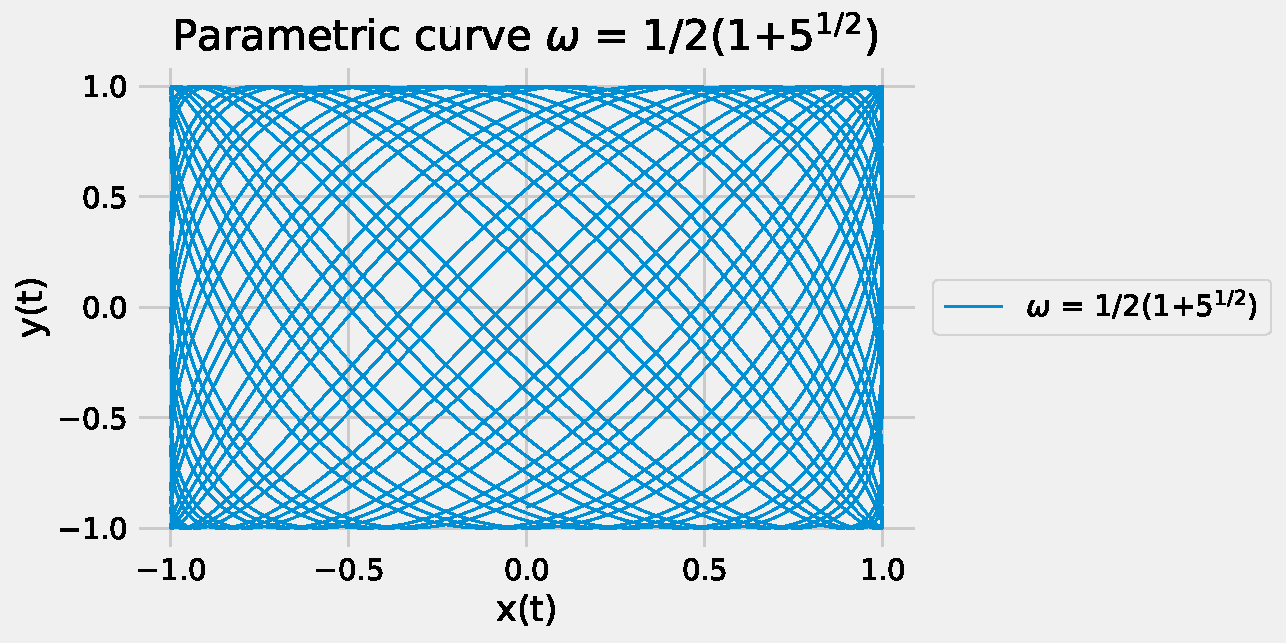
\includegraphics[width = 12 cm]{src/parametricw6.pdf}
    \caption{Lissajous figure with a "frequency" of $\omega = 1/2(1+5^{1/2})$. The frequency is an irrational number. The Lissajous figures seem to exhibit dynamical behavior based on rational or irrational frequencies. Theories of dynamical system has stated that irrational initial conditions in a domain will strongly imply attraction towards a chaotic orbit, while rational numbers heads towards a period fixed points. After larger time steps, the rational plots tend to stay the same no matter the change in time scale. These rational plots appear to be in periodic orbits, while plots of irrational frequencies increase their dynamical behavior after more iterations in time.}
    \label{fig:my_label}
\end{figure}

\clearpage


\section*{Orbital transitions}

First, let's define the parameters/constants/variables needed for the system.\\

\begin{tabular}{l|l|l}
    Variable & Value &  Description \\ 
    \hline 
     $m_s$ &  & mass of satellite \\
     $m_e$ & 5.98*$10^{24} $ Kg & mass of Earth \\
     $G$ & 6.67*$10^{-11}$ $m^3$/(Kg*$s^2$) & Gravitational constant \\
     $\epsilon_1$ & 0.9656 & Initial eccentricity \\
     $\delta$ & 0.01 & Percantage of reduction \\
     $r_{\text{min}}$ & 6600 km & minimum distance from focal/apogee 
\end{tabular} 
\\
\\
After the first orbit, each successive orbit the speed of the satellite will reduce about $\delta$*initial velocity, $v_1$, for every successive orbit passing through Earth's atmosphere around 200 km above Earth's surface. Take in account the energy of the first orbit, we could find the initial velocity as $r_{\text{min}}$. Note: $\mu$ = G*$m_e$.
\begin{align*}
    E = & \frac{m_sv_1^2}{2} - \frac{m_s\mu}{r_{min}} ; \ \ \text{where E =} \frac{-m_s\mu}{2a_1} 
    \end{align*}
    \begin{align*}
         \frac{-m_s\mu}{2a_1} = &  \frac{m_sv_1^2}{2} - \frac{m_s\mu}{r_{min}} \\
           \frac{v_1^2}{2} = & \frac{\mu}{r_{min}}  - \frac{\mu}{2a_1} \\
   v_1 =& \sqrt{\mu(\frac{2}{r_{min}}  - \frac{1}{a_1})}
\end{align*}
After each orbit n, the velocity will be reduced by $\delta v_n$, where $v_{n+1} = v_n(1-\delta)$. Solving for the conic section $\alpha$, we can find the first semimajor axis of the first orbit $a_1$ and all following semimajor axis by $a_{n}$ = $r_{min}$/(1-$\epsilon_n$). 
All we need now is how to find the eccentricity varies after each successive orbit then computationally find the number of orbits and time it takes after each successive iterations. 
\begin{align*}
    \epsilon_{n+1} = &  \sqrt{1+\frac{2E_{n+1}l_{n+1}^2}{m_s(\mu m_s)^2}}; l_{n+1} = m_sv_{n+1}r_{min} \\
    \epsilon_{n+1} = &  \sqrt{1+\frac{2l_{n+1}^2}{m_s(\mu m_s)^2}(\frac{m_sv_{n+1}^2}{2} - \frac{m_s\mu}{r_{min}})} \\
    \epsilon_{n+1} = &  \sqrt{1+\frac{2( m_sv_{n+1}r_{min})^2}{(\mu m_s)^2}(\frac{v_{n+1}^2}{2} - \frac{\mu}{r_{min}})} \\
    \epsilon_{n+1} = &  \sqrt{1+\frac{(v_{n+1}r_{min})^2}{\mu^2}(v_{n+1}^2 - \frac{2\mu}{r_{min}})} \\
    \epsilon_{n+1} = &  \sqrt{1+(\frac{v_{n+1}r_{min}}{\mu})^2(v_{n+1}^2 - \frac{2\mu}{r_{min}})} 
\end{align*}
Computationally code this in a loop til the eccentricity approximately reaches a circular orbit when $\epsilon_{n+1} < 1/7$. 
a.) Based on the calculations, the satellite took 28 orbits to circularize.
b.) Using Kepler's third law and each successive change in semimajor axis, we approximated the time the satellite to complete the transition into a circular orbit to be 20.75 days.  

\begin{figure}[H]
    \centering
    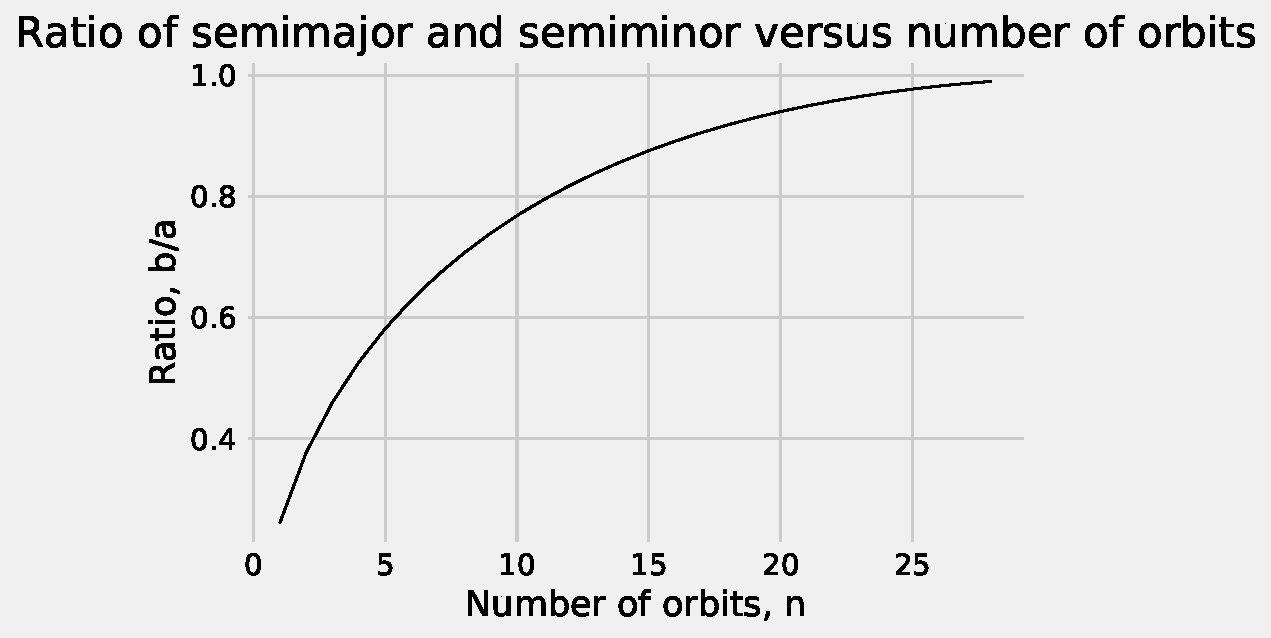
\includegraphics[width = 12 cm]{src/Ratio.pdf}
    \caption{Ratio between semiminor axis and semimajor axis of a transition form an elliptical orbit to circular orbit. The satellite took 28 orbits to circularize. As the satellite approaches a circular orbit, the ratio is one signaling the approximate number of orbit transitions for the satellite to be in a circular orbit. The semiminor axis was found by each successive change in $r_{max}$, b = $\sqrt{r_{min}r_{max}}$.}
    \label{fig:my_label}
\end{figure}
d.) At the apogee, or $r_{max}$, the velocity was at 6238 km/s on the last orbit compared to 190.7 in the first orbit. As each successive orbit, the speed of the apogee increases due to the conservation of angular momentum. For angular momentum to be conserved as the satellite transitions into a smaller radial orbit, the faster the satellite has to go for angular momentum to be a constant.

\clearpage
\section*{Simple Pendulum}
    Defining our coordinate system as x= rsin($\phi$), y = -rcos($\phia$), where r is the length of the string. Setting up the equations 
    from the Lagrangian, the equation of motion for a simple pendulum is L = 1/2 m($v_x^2$+$v_y^2$)-mgy = 1/2 m(($r^2cos^2(\phi)$ 
    $\dot{\phi}^2$+$r^2sin^2(\phi)$ $\dot{\phi}^2$) + mgr$cos(\phi)$ = 1/2 m($r^2$ $\Dot{\phi}^2$) + mgr$cos(\phi)$. Plugging into the 
    Lagrangian equation with $\phi$ as our only generalized coordinate since there is no change in r or $\dot{r}$. 
    
    
    \begin{align*}
        \frac{d}{dt} \frac{dL}{d(\Dot{\phi})} = & \ \frac{dL}{d\phi} \\
        m(r^2 \ddot{\phi}) = & \  mgrcos(\phi) \\
        \ddot{\phi} = & \ -\frac{g}{r}sin(\phi)
    \end{align*}
    For small angles, we can approximate sin($\phi$) $\approx $ $\phi$ due to small angles $\phi^2 \ll 1$. For the nonlinear case, at large angles, we will have to find a computational analytic solution. For both cases, we can use ODE system of equations like Runge-Kutta to solve for the solution of the simple pendulum. In python, we use odeint from scipy to find the motion of $\phi$(t). 
\begin{figure}[H]
    \centering
    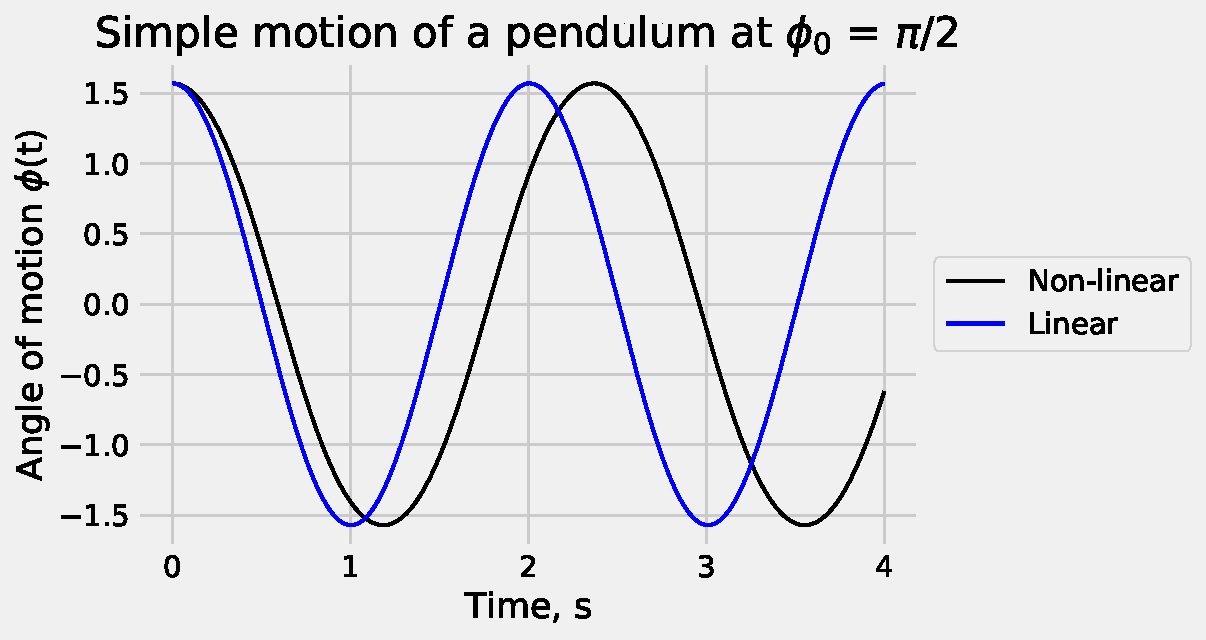
\includegraphics[width = 12 cm]{src/Pendulum.pdf}
    \caption{Motion of the simple pendulum at an initial condition of $\phi_0 = \pi/2$. At the threshold of $\pi$/2, the pendulum for the nonlinear case starts to take a longer time to  oscillate compared to approximation.}
    \label{fig:my_label}
\end{figure}

\begin{figure}[H]
    \centering
    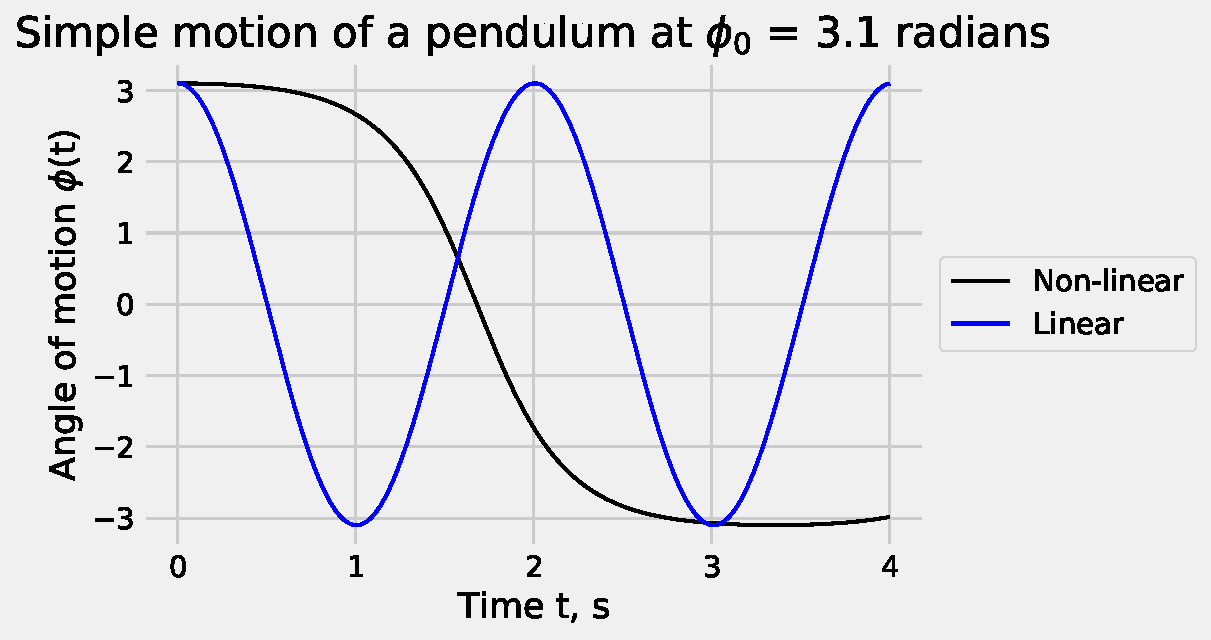
\includegraphics[width = 12 cm]{src/PendulumPb.pdf}
    \caption{Motion of the simple pendulum at an initial condition of $\phi_0 =$ 3.1 radians. At large angles, the time the pendulum takes to make a full periodic swing is even longer. This is because only gravity is giving the pendulum enough force to make an oscillation.}
    \label{fig:my_label}
\end{figure}
By plotting ODE system for set of initial conditions of $\phi_0$ from 0.1 to 3.1 radians. At an initial condition of $\phi_0 = 0.55$ radians does the nonlinear simple pendulum diverges 2 percent of the natural frequency of the linear pendulum. After 0.55 radians does the nonlinear case exponentially increases. 
\begin{figure}[H]
    \centering
    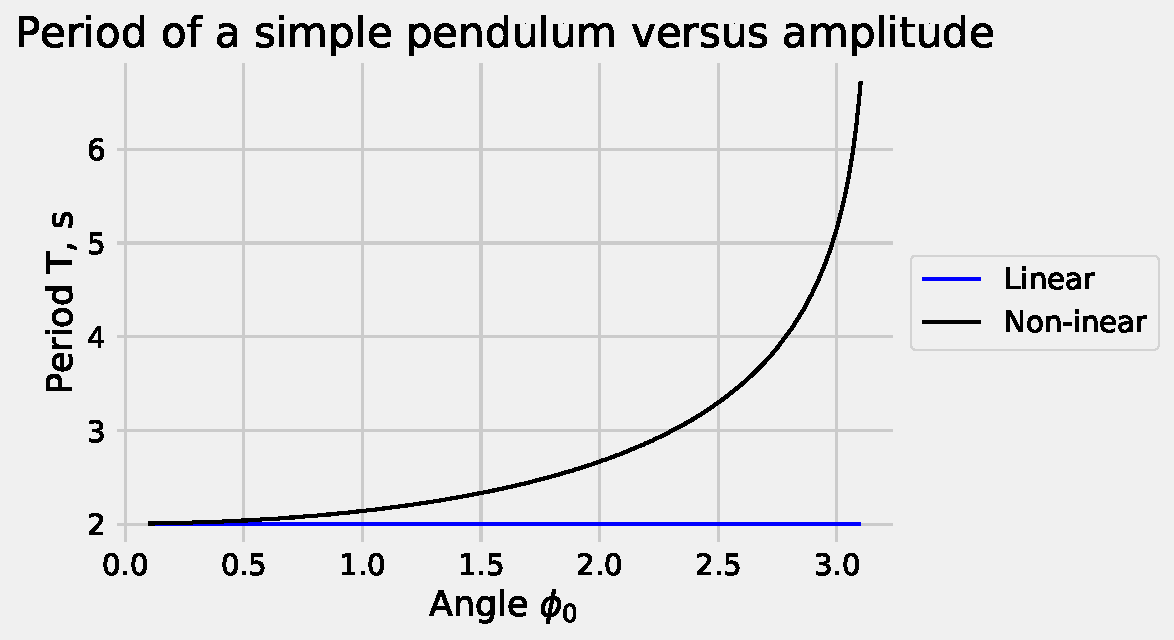
\includegraphics[width = 12 cm]{src/PendulumPc.pdf}
    \caption{Period of oscillation comparison between the nonlinear and linear motion of a simple pendulum. At angle 0.55 radians, the nonlinear case starts to diverge from the linear frequency of $\omega = 2\pi \sqrt{\frac{g}{r}}$, by two percent. The difference between linear and nonlinear exponentially increases after 0.55 radians.  }
    \label{fig:my_label}
\end{figure}
\end{document}